\documentclass[11pt]{article}

\usepackage{times,mathptm}
\usepackage{pifont}
\usepackage{exscale}
\usepackage{latexsym}
\usepackage{amsmath}
\usepackage{amssymb}
\usepackage{amsthm}
\usepackage{epsfig}
\usepackage{tikz}


\textwidth 6.5in
\textheight 9in
\oddsidemargin -0.0in
\topmargin -0.0in

\parindent 0pt     % How much the first word of a paragraph is indented. 
\parskip 0pt	   % How much extra space to leave between paragraphs.

\begin{document}

\begin{center}             % If you only centering 1 line use \centerline{}
\begin{LARGE}
{\bf Finite Automata Homework 2}
\end{LARGE}
\vskip 0.25cm      % vertical skip (0.25 cm)

Due: Thursday, Sep 17\\  % force new line
Alexander Powell
\end{center}

\begin{enumerate}

\item Below is an NFA with six states that accepts the language 

$ L = \{$ $w$ $|$ $w$ contains an even number of 0s, or contains exactly two 1s $\} $

\begin{center}
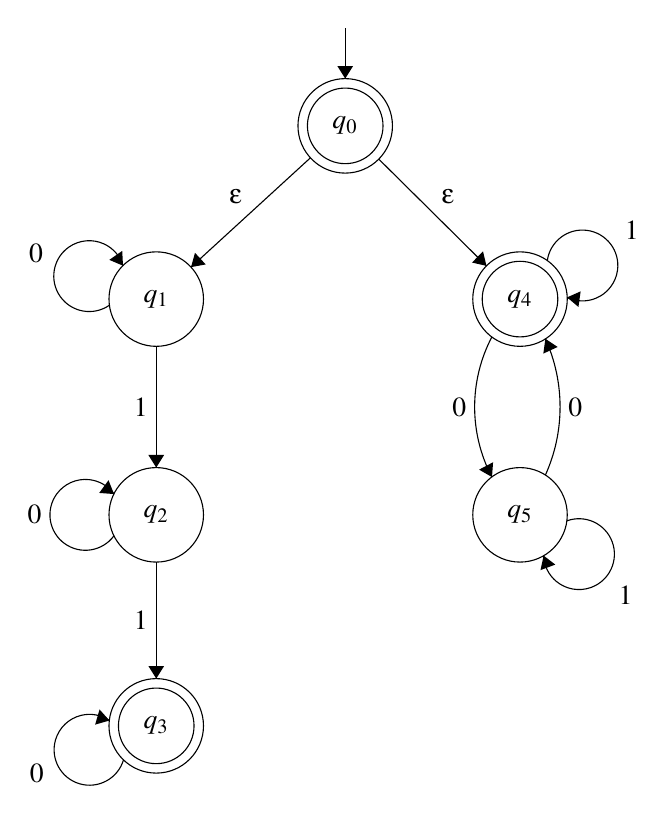
\begin{tikzpicture}[scale=0.2]
\tikzstyle{every node}+=[inner sep=0pt]
\draw [black] (38.8,-11.7) circle (3);
\draw (38.8,-11.7) node {$q_0$};
\draw [black] (38.8,-11.7) circle (2.4);
\draw [black] (26.8,-22.7) circle (3);
\draw (26.8,-22.7) node {$q_1$};
\draw [black] (49.9,-22.7) circle (3);
\draw (49.9,-22.7) node {$q_4$};
\draw [black] (49.9,-22.7) circle (2.4);
\draw [black] (49.9,-36.4) circle (3);
\draw (49.9,-36.4) node {$q_5$};
\draw [black] (26.8,-36.4) circle (3);
\draw (26.8,-36.4) node {$q_2$};
\draw [black] (26.8,-49.8) circle (3);
\draw (26.8,-49.8) node {$q_3$};
\draw [black] (26.8,-49.8) circle (2.4);
\draw [black] (40.93,-13.81) -- (47.77,-20.59);
\fill [black] (47.77,-20.59) -- (47.55,-19.67) -- (46.85,-20.38);
\draw (45.32,-16.72) node [above] {$\epsilon$};
\draw [black] (36.59,-13.73) -- (29.01,-20.67);
\fill [black] (29.01,-20.67) -- (29.94,-20.5) -- (29.26,-19.76);
\draw (31.84,-16.71) node [above] {$\epsilon$};
\draw [black] (38.8,-5.5) -- (38.8,-8.7);
\fill [black] (38.8,-8.7) -- (39.3,-7.9) -- (38.3,-7.9);
\draw [black] (48.116,-34.003) arc (-152.30454:-207.69546:9.582);
\fill [black] (48.12,-34) -- (48.19,-33.06) -- (47.3,-33.53);
\draw (46.52,-29.55) node [left] {$0$};
\draw [black] (51.509,-25.22) arc (24.36031:-24.36031:10.497);
\fill [black] (51.51,-25.22) -- (51.38,-26.16) -- (52.29,-25.74);
\draw (52.94,-29.55) node [right] {$0$};
\draw [black] (23.836,-23.082) arc (305.07968:17.07968:2.25);
\draw (19.65,-19.78) node [left] {$0$};
\fill [black] (24.69,-20.58) -- (24.64,-19.64) -- (23.82,-20.21);
\draw [black] (24.12,-37.723) arc (-36:-324:2.25);
\draw (19.55,-36.4) node [left] {$0$};
\fill [black] (24.12,-35.08) -- (23.77,-34.2) -- (23.18,-35.01);
\draw [black] (24.724,-51.949) arc (-16.27496:-304.27496:2.25);
\draw (19.69,-52.85) node [left] {$0$};
\fill [black] (23.83,-49.46) -- (23.2,-48.76) -- (22.92,-49.72);
\draw [black] (26.8,-25.7) -- (26.8,-33.4);
\fill [black] (26.8,-33.4) -- (27.3,-32.6) -- (26.3,-32.6);
\draw (26.3,-29.55) node [left] {$1$};
\draw [black] (26.8,-39.4) -- (26.8,-46.8);
\fill [black] (26.8,-46.8) -- (27.3,-46) -- (26.3,-46);
\draw (26.3,-43.1) node [left] {$1$};
\draw [black] (51.632,-20.265) arc (172.30076:-115.69924:2.25);
\draw (56.52,-18.33) node [right] {$1$};
\fill [black] (52.89,-22.59) -- (53.61,-23.2) -- (53.75,-22.21);
\draw [black] (52.863,-36.786) arc (110.30993:-177.69007:2.25);
\draw (56.13,-41.48) node [right] {$1$};
\fill [black] (51.4,-38.99) -- (51.2,-39.91) -- (52.14,-39.56);
\end{tikzpicture}
\end{center}

The DFA for this language is shown below with eight states.  

\begin{center}
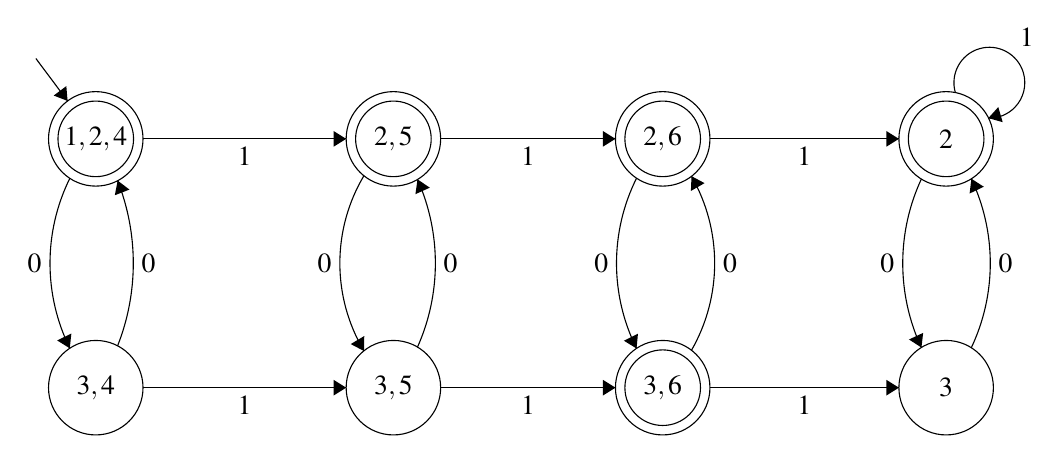
\begin{tikzpicture}[scale=0.2]
\tikzstyle{every node}+=[inner sep=0pt]
\draw [black] (13.1,-9.8) circle (3);
\draw (13.1,-9.8) node {${1,2,4}$};
\draw [black] (13.1,-9.8) circle (2.4);
\draw [black] (32,-9.8) circle (3);
\draw (32,-9.8) node {${2,5}$};
\draw [black] (32,-9.8) circle (2.4);
\draw [black] (49.1,-9.8) circle (3);
\draw (49.1,-9.8) node {${2,6}$};
\draw [black] (49.1,-9.8) circle (2.4);
\draw [black] (67.1,-9.8) circle (3);
\draw (67.1,-9.8) node {${2}$};
\draw [black] (67.1,-9.8) circle (2.4);
\draw [black] (13.1,-25.6) circle (3);
\draw (13.1,-25.6) node {${3,4}$};
\draw [black] (32,-25.6) circle (3);
\draw (32,-25.6) node {${3,5}$};
\draw [black] (49.1,-25.6) circle (3);
\draw (49.1,-25.6) node {${3,6}$};
\draw [black] (49.1,-25.6) circle (2.4);
\draw [black] (67.1,-25.6) circle (3);
\draw (67.1,-25.6) node {${3}$};
\draw [black] (11.455,-23.1) arc (-153.69998:-206.30002:12.188);
\fill [black] (11.45,-23.1) -- (11.55,-22.16) -- (10.65,-22.6);
\draw (9.69,-17.7) node [left] {$0$};
\draw [black] (14.485,-12.455) arc (21.54237:-21.54237:14.285);
\fill [black] (14.49,-12.45) -- (14.31,-13.38) -- (15.24,-13.02);
\draw (15.98,-17.7) node [right] {$0$};
\draw [black] (30.131,-23.265) arc (-149.22517:-210.77483:10.877);
\fill [black] (30.13,-23.27) -- (30.15,-22.32) -- (29.29,-22.83);
\draw (28.1,-17.7) node [left] {$0$};
\draw [black] (47.442,-23.109) arc (-153.45771:-206.54229:12.104);
\fill [black] (47.44,-23.11) -- (47.53,-22.17) -- (46.64,-22.62);
\draw (45.67,-17.7) node [left] {$0$};
\draw [black] (65.527,-23.054) arc (-155.06253:-204.93747:12.698);
\fill [black] (65.53,-23.05) -- (65.64,-22.12) -- (64.74,-22.54);
\draw (63.84,-17.7) node [left] {$0$};
\draw [black] (33.528,-12.374) arc (24.10254:-24.10254:13.042);
\fill [black] (33.53,-12.37) -- (33.4,-13.31) -- (34.31,-12.9);
\draw (35.16,-17.7) node [right] {$0$};
\draw [black] (50.925,-12.169) arc (29.86908:-29.86908:11.105);
\fill [black] (50.93,-12.17) -- (50.89,-13.11) -- (51.76,-12.61);
\draw (52.9,-17.7) node [right] {$0$};
\draw [black] (68.695,-12.332) arc (25.35265:-25.35265:12.536);
\fill [black] (68.7,-12.33) -- (68.59,-13.27) -- (69.49,-12.84);
\draw (70.4,-17.7) node [right] {$0$};
\draw [black] (16.1,-9.8) -- (29,-9.8);
\fill [black] (29,-9.8) -- (28.2,-9.3) -- (28.2,-10.3);
\draw (22.55,-10.3) node [below] {$1$};
\draw [black] (35,-9.8) -- (46.1,-9.8);
\fill [black] (46.1,-9.8) -- (45.3,-9.3) -- (45.3,-10.3);
\draw (40.55,-10.3) node [below] {$1$};
\draw [black] (52.1,-9.8) -- (64.1,-9.8);
\fill [black] (64.1,-9.8) -- (63.3,-9.3) -- (63.3,-10.3);
\draw (58.1,-10.3) node [below] {$1$};
\draw [black] (16.1,-25.6) -- (29,-25.6);
\fill [black] (29,-25.6) -- (28.2,-25.1) -- (28.2,-26.1);
\draw (22.55,-26.1) node [below] {$1$};
\draw [black] (35,-25.6) -- (46.1,-25.6);
\fill [black] (46.1,-25.6) -- (45.3,-25.1) -- (45.3,-26.1);
\draw (40.55,-26.1) node [below] {$1$};
\draw [black] (52.1,-25.6) -- (64.1,-25.6);
\fill [black] (64.1,-25.6) -- (63.3,-25.1) -- (63.3,-26.1);
\draw (58.1,-26.1) node [below] {$1$};
\draw [black] (9.3,-4.7) -- (11.31,-7.39);
\fill [black] (11.31,-7.39) -- (11.23,-6.45) -- (10.43,-7.05);
\draw [black] (67.686,-6.87) arc (196.43141:-91.56859:2.25);
\draw (72.22,-3.95) node [above] {$1$};
\fill [black] (69.78,-8.48) -- (70.69,-8.74) -- (70.41,-7.78);
\end{tikzpicture}
\end{center}

\newpage

\item The given NFA is shown below.  

\begin{center}
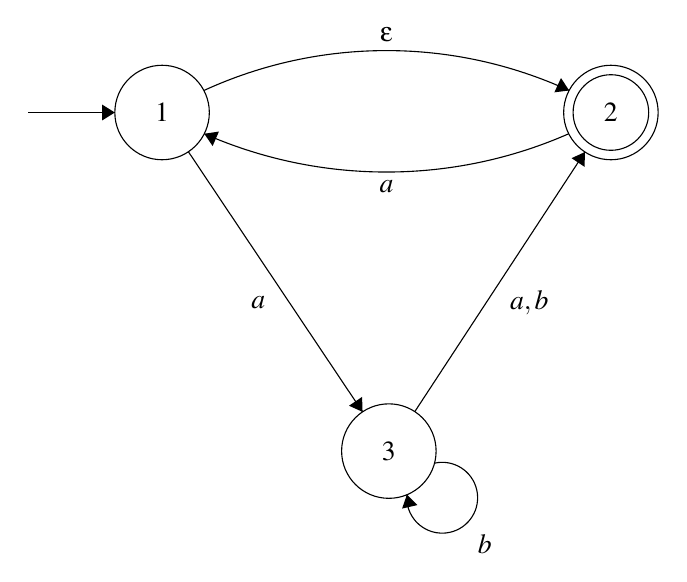
\begin{tikzpicture}[scale=0.2]
\tikzstyle{every node}+=[inner sep=0pt]
\draw [black] (21.6,-12.6) circle (3);
\draw (21.6,-12.6) node {$1$};
\draw [black] (50.1,-12.6) circle (3);
\draw (50.1,-12.6) node {$2$};
\draw [black] (50.1,-12.6) circle (2.4);
\draw [black] (36,-34.1) circle (3);
\draw (36,-34.1) node {$3$};
\draw [black] (23.27,-15.09) -- (34.33,-31.61);
\fill [black] (34.33,-31.61) -- (34.3,-30.66) -- (33.47,-31.22);
\draw (28.19,-24.69) node [left] {$a$};
\draw [black] (37.65,-31.59) -- (48.45,-15.11);
\fill [black] (48.45,-15.11) -- (47.6,-15.5) -- (48.43,-16.05);
\draw (43.66,-24.67) node [right] {$a,b$};
\draw [black] (47.422,-13.949) arc (-66.26289:-113.73711:28.747);
\fill [black] (24.28,-13.95) -- (24.81,-14.73) -- (25.21,-13.81);
\draw (35.85,-16.88) node [below] {$a$};
\draw [black] (24.253,-11.203) arc (114.67083:65.32917:27.783);
\fill [black] (47.45,-11.2) -- (46.93,-10.41) -- (46.51,-11.32);
\draw (35.85,-8.17) node [above] {$\epsilon$};
\draw [black] (38.888,-34.869) arc (102.81407:-185.18593:2.25);
\draw (41.62,-40) node [right] {$b$};
\fill [black] (37.15,-36.86) -- (36.84,-37.75) -- (37.81,-37.53);
\draw [black] (13.1,-12.6) -- (18.6,-12.6);
\fill [black] (18.6,-12.6) -- (17.8,-12.1) -- (17.8,-13.1);
\end{tikzpicture}
\end{center}

Converting to a DFA, we initially get a graph like the one shown below.  

\begin{center}
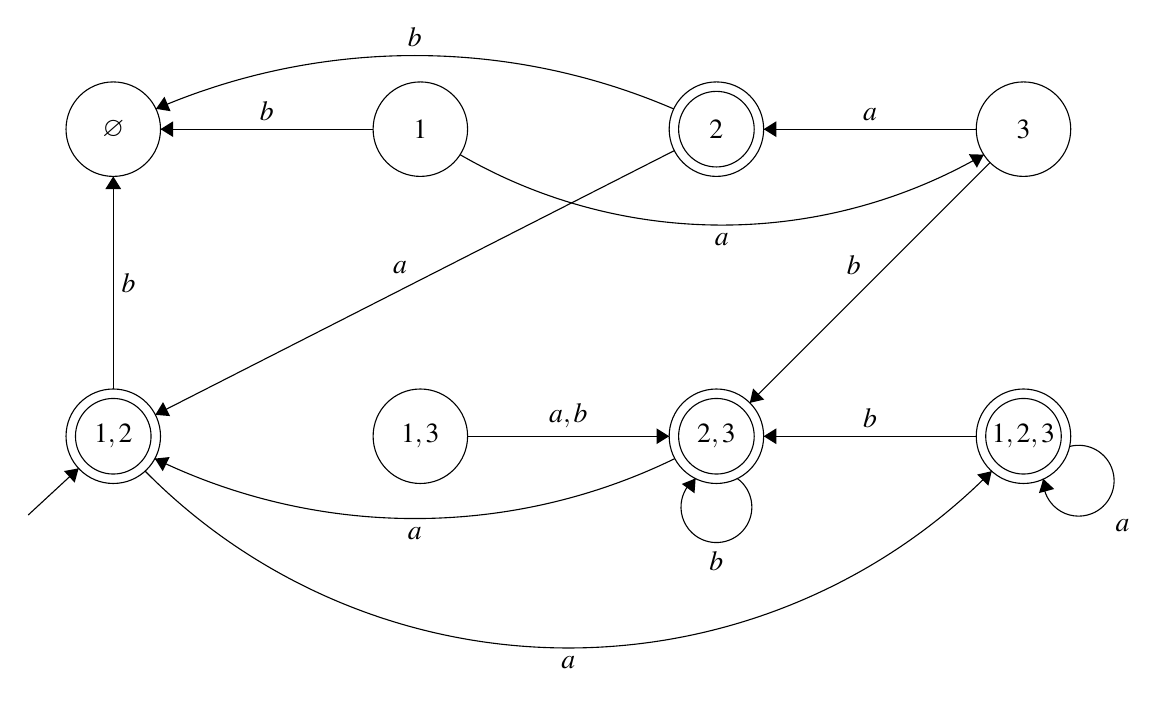
\begin{tikzpicture}[scale=0.2]
\tikzstyle{every node}+=[inner sep=0pt]
\draw [black] (11.1,-8.7) circle (3);
\draw (11.1,-8.7) node {$\varnothing$};
\draw [black] (30.6,-8.7) circle (3);
\draw (30.6,-8.7) node {${1}$};
\draw [black] (49.4,-8.7) circle (3);
\draw (49.4,-8.7) node {${2}$};
\draw [black] (49.4,-8.7) circle (2.4);
\draw [black] (68.9,-8.7) circle (3);
\draw (68.9,-8.7) node {${3}$};
\draw [black] (11.1,-28.2) circle (3);
\draw (11.1,-28.2) node {${1,2}$};
\draw [black] (11.1,-28.2) circle (2.4);
\draw [black] (30.6,-28.2) circle (3);
\draw (30.6,-28.2) node {${1,3}$};
\draw [black] (49.4,-28.2) circle (3);
\draw (49.4,-28.2) node {${2,3}$};
\draw [black] (49.4,-28.2) circle (2.4);
\draw [black] (68.9,-28.2) circle (3);
\draw (68.9,-28.2) node {${1,2,3}$};
\draw [black] (68.9,-28.2) circle (2.4);
\draw [black] (27.6,-8.7) -- (14.1,-8.7);
\fill [black] (14.1,-8.7) -- (14.9,-9.2) -- (14.9,-8.2);
\draw (20.85,-8.2) node [above] {$b$};
\draw [black] (11.1,-25.2) -- (11.1,-11.7);
\fill [black] (11.1,-11.7) -- (10.6,-12.5) -- (11.6,-12.5);
\draw (11.6,-18.45) node [right] {$b$};
\draw [black] (46.73,-10.06) -- (13.77,-26.84);
\fill [black] (13.77,-26.84) -- (14.71,-26.92) -- (14.26,-26.03);
\draw (29.31,-17.95) node [above] {$a$};
\draw [black] (13.81,-7.415) arc (113.303:66.697:41.558);
\fill [black] (13.81,-7.41) -- (14.74,-7.56) -- (14.35,-6.64);
\draw (30.25,-3.52) node [above] {$b$};
\draw [black] (66.376,-10.32) arc (-59.89385:-120.10615:33.146);
\fill [black] (66.38,-10.32) -- (65.43,-10.29) -- (65.94,-11.15);
\draw (49.75,-15.29) node [below] {$a$};
\draw [black] (71.816,-28.852) arc (105.13083:-182.86917:2.25);
\draw (74.72,-33.86) node [right] {$a$};
\fill [black] (70.16,-30.91) -- (69.88,-31.81) -- (70.85,-31.55);
\draw [black] (65.9,-28.2) -- (52.4,-28.2);
\fill [black] (52.4,-28.2) -- (53.2,-28.7) -- (53.2,-27.7);
\draw (59.15,-27.7) node [above] {$b$};
\draw [black] (50.723,-30.88) arc (54:-234:2.25);
\draw (49.4,-35.45) node [below] {$b$};
\fill [black] (48.08,-30.88) -- (47.2,-31.23) -- (48.01,-31.82);
\draw [black] (46.758,-29.62) arc (-64.02351:-115.97649:37.69);
\fill [black] (13.74,-29.62) -- (14.24,-30.42) -- (14.68,-29.52);
\draw (30.25,-33.93) node [below] {$a$};
\draw [black] (66.879,-30.416) arc (-44.65142:-135.34858:37.783);
\fill [black] (66.88,-30.42) -- (65.96,-30.63) -- (66.67,-31.34);
\draw (40,-42.14) node [below] {$a$};
\draw [black] (65.9,-8.7) -- (52.4,-8.7);
\fill [black] (52.4,-8.7) -- (53.2,-9.2) -- (53.2,-8.2);
\draw (59.15,-8.2) node [above] {$a$};
\draw [black] (33.6,-28.2) -- (46.4,-28.2);
\fill [black] (46.4,-28.2) -- (45.6,-27.7) -- (45.6,-28.7);
\draw (40,-27.7) node [above] {$a,b$};
\draw [black] (66.78,-10.82) -- (51.52,-26.08);
\fill [black] (51.52,-26.08) -- (52.44,-25.87) -- (51.73,-25.16);
\draw (58.13,-17.97) node [above] {$b$};
\draw [black] (5.7,-33.2) -- (8.9,-30.24);
\fill [black] (8.9,-30.24) -- (7.97,-30.41) -- (8.65,-31.15);
\end{tikzpicture}
\end{center}

\newpage

By eliminating nodes that only have outgoing arcs and nodes that are dead end states, we can simplify the DFA to the following:

\begin{center}
\begin{tikzpicture}[scale=0.2]
\tikzstyle{every node}+=[inner sep=0pt]
\draw [black] (19.6,-14) circle (3);
\draw (19.6,-14) node {${1,2}$};
\draw [black] (19.6,-14) circle (2.4);
\draw [black] (54.9,-14) circle (3);
\draw (54.9,-14) node {${1,2,3}$};
\draw [black] (54.9,-14) circle (2.4);
\draw [black] (37.8,-36.9) circle (3);
\draw (37.8,-36.9) node {${2,3}$};
\draw [black] (37.8,-36.9) circle (2.4);
\draw [black] (35.93,-34.55) -- (21.47,-16.35);
\fill [black] (21.47,-16.35) -- (21.57,-17.29) -- (22.36,-16.66);
\draw (29.26,-24.03) node [right] {$a$};
\draw [black] (53.11,-16.4) -- (39.59,-34.5);
\fill [black] (39.59,-34.5) -- (40.47,-34.15) -- (39.67,-33.56);
\draw (45.77,-24.06) node [left] {$b$};
\draw [black] (22.188,-12.485) arc (117.69576:62.30424:32.407);
\fill [black] (52.31,-12.48) -- (51.84,-11.67) -- (51.37,-12.56);
\draw (37.25,-8.27) node [above] {$a$};
\draw [black] (12.1,-7.3) -- (17.36,-12);
\fill [black] (17.36,-12) -- (17.1,-11.1) -- (16.43,-11.84);
\draw [black] (39.123,-39.58) arc (54:-234:2.25);
\draw (37.8,-44.15) node [below] {$b$};
\fill [black] (36.48,-39.58) -- (35.6,-39.93) -- (36.41,-40.52);
\draw [black] (56.842,-11.729) arc (167.19859:-120.80141:2.25);
\draw (61.84,-10.39) node [right] {$a$};
\fill [black] (57.88,-14.16) -- (58.55,-14.82) -- (58.77,-13.85);
\end{tikzpicture}
\end{center}

The language recognized by the finite automata can be defined by $L$ where, $L = \{$ $w$ $|$ $w$ does not begin with b and $w$ does not contain the substring bab $\}$.  

\item To show that $B$ is a regular language, we simply need to show that a DFA can be constructed to accept all states of $B$.  We see this DFA below.  

\begin{center}
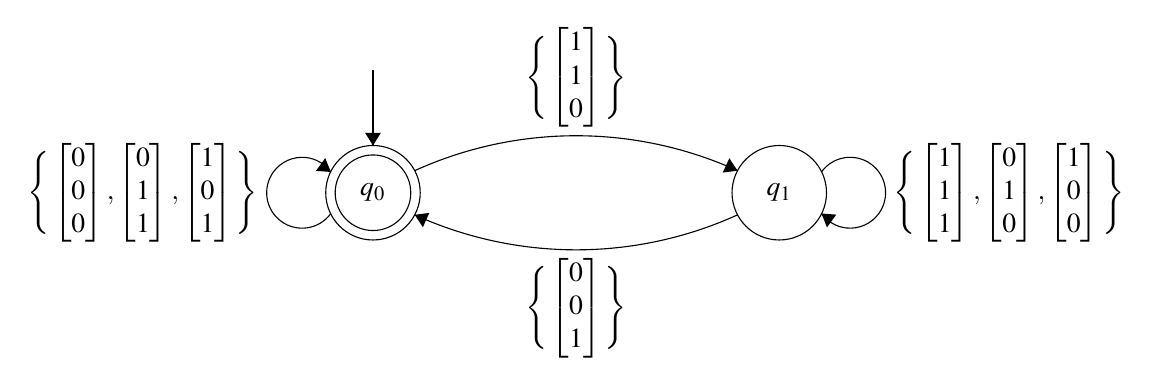
\begin{tikzpicture}[scale=0.2]
\tikzstyle{every node}+=[inner sep=0pt]
\draw [black] (26.2,-21.3) circle (3);
\draw (26.2,-21.3) node {$q_0$};
\draw [black] (26.2,-21.3) circle (2.4);
\draw [black] (52,-21.3) circle (3);
\draw (52,-21.3) node {$q_1$};
\draw [black] (23.52,-22.623) arc (324:36:2.25);
\draw (18.95,-21.3) node [left] {$ \Bigg\{ \begin{bmatrix}0\\0\\0\end{bmatrix},\begin{bmatrix}0\\1\\1\end{bmatrix} ,\begin{bmatrix}1\\0\\1\end{bmatrix} \Bigg\} $};
\fill [black] (23.52,-19.98) -- (23.17,-19.1) -- (22.58,-19.91);
\draw [black] (54.68,-19.977) arc (144:-144:2.25);
\draw (59.25,-21.3) node [right] {$ \Bigg\{ \begin{bmatrix}1\\1\\1\end{bmatrix},\begin{bmatrix}0\\1\\0\end{bmatrix} ,\begin{bmatrix}1\\0\\0\end{bmatrix} \Bigg\} $};
\fill [black] (54.68,-22.62) -- (55.03,-23.5) -- (55.62,-22.69);
\draw [black] (28.85,-19.898) arc (114.41914:65.58086:24.794);
\fill [black] (49.35,-19.9) -- (48.83,-19.11) -- (48.41,-20.02);
\draw (39.1,-17.18) node [above] {$ \Bigg\{  \begin{bmatrix}1\\1\\0\end{bmatrix}  \Bigg\} $};
\draw [black] (49.351,-22.704) arc (-65.53877:-114.46123:24.757);
\fill [black] (28.85,-22.7) -- (29.37,-23.49) -- (29.78,-22.58);
\draw (39.1,-25.43) node [below] {$ \Bigg\{  \begin{bmatrix}0\\0\\1\end{bmatrix}  \Bigg\} $};
\draw [black] (26.2,-13.5) -- (26.2,-18.3);
\fill [black] (26.2,-18.3) -- (26.7,-17.5) -- (25.7,-17.5);
\end{tikzpicture}
\end{center}

Therefore, $B$ is in fact a regular language.  

\end{enumerate}

\end{document}









